\documentclass[12pt]{article}

\bibliography{sbc-template}

\usepackage{graphicx}
\usepackage{indentfirst}
\usepackage[utf8]{inputenc}
\usepackage{listings}
\usepackage{sbc-template}
\usepackage{url}

\lstset{language=[LaTeX]TeX,
        basicstyle=\ttfamily,
        columns=fullflexible,
        keepspaces=true}

\sloppy

\title{Relatório do Projeto: CPU RISC-V 32 Bits}
\author{Andrés Gonzalez Vilhena\\
        David Moreira Jacinto da Silva\\
        Lucas da Silva Inocencio}

\address{Escola Politécnica da Universidade Federal do Rio de Janeiro (UFRJ)\\
  Rio de Janeiro -- RJ -- Brasil
\email{agv1@poli.ufrj.br, davidmoreirajacinto.20222@poli.ufrj.br}
\email{lucas.inocencio@poli.ufrj.br}
}

\begin{document}

\maketitle

\begin{abstract}
This project aims to design and implement a 32-bit RISC-V Central Processing Unit (CPU) following the RV32I instruction set architecture. The CPU's microarchitecture will be based on a 5-stage pipeline, utilizing VHDL blocks in the LogiSIM-Evolution simulator. The instruction and data memories will be distinct, delivering one word per cycle, and will be modified to enable asynchronous data loading using the ROM and RAM memories provided by LogiSIM-Evolution. The CPU will be constructed using VHDL blocks and organized into a 5-stage pipeline for enhanced instruction throughput and overall performance. The instruction and data memories will be optimized for asynchronous data loading to ensure seamless operation without compromising the CPU's internal state.
\end{abstract}

\section{Enunciado}

Projetar e implementar uma CPU RISC-V de 32 Bits (RV32I) cuja microarquitetura seja baseada em um pipeline com ao menos 5 estágios, a implementação deve ser realizada usando blocos VHDL no simulador LogiSIM-Evolution. As memórias de instruções e dados são distintas e entregam cada uma palavra por ciclo, além disso essas memórias devem ser modificadas para permitir carga de dados assíncrona (pode usar as memórias ROM e RAM do LogiSIM-Evolution). A CPU deve ser adaptada para não operar durante essa carga de dados (manter seu estado interno corrente), além de possuir um sinal de reset. Para esta tarefa apenas o pipeline de inteiros será implementado, sem modo supervisor (S Mode , especificamente as instruções a seguir devem ser suportadas:

\begin{itemize}
    \item add, addi, auipc e sub
    \item and, andi, or, ori, xor e xor
    \item sll, slli, srl e srli
    \item lw, lui e sw
    \item jal, jalr, beq e bne
\end{itemize}

Desaconselho fortemente o uso de blocos combinacionais de múltiplos bits do LogiSIM-Evolution, em especial os de ALU.

\section{Introdução}
Este projeto tem como objetivo projetar e implementar uma Unidade Central de Processamento (CPU) baseada na arquitetura RISC-V de 32 bits (RV32I). A CPU será desenvolvida utilizando a linguagem VHDL e será implementada em um pipeline de 5 estágios, proporcionando melhor desempenho e maior eficiência na execução de instruções.

A arquitetura RISC-V é uma arquitetura de conjunto de instruções (ISA) aberta e livre, que tem ganhado destaque na indústria e na academia devido à sua simplicidade e facilidade de implementação. O conjunto de instruções RV32I representa a base dessa arquitetura, oferecendo um conjunto sólido e funcional de instruções para operações inteiras.

O pipeline é uma técnica utilizada para melhorar o desempenho da CPU, permitindo a execução de múltiplas instruções em paralelo, dividindo o processo de execução em etapas sequenciais. Neste projeto, o pipeline será composto por cinco estágios: busca de instrução (IF - Instruction Fetch), decodificação de instrução (ID - Instruction Decode), execução (EX - Execution), acesso à memória (MEM - Memory Access) e escrita de resultados (WB - Write Back).

Para viabilizar o funcionamento adequado da CPU, serão utilizadas duas memórias distintas: uma para as instruções (IMEM) e outra para os dados (DMEM). A abordagem de leitura de palavras por ciclo será adotada, proporcionando maior eficiência na busca e execução das instruções.

Um dos desafios deste projeto será a modificação das memórias para permitir a carga assíncrona de dados, possibilitando a operação contínua da CPU durante esse processo, enquanto mantém seu estado interno corrente. Além disso, será implementado um sinal de reset para reiniciar a CPU, garantindo seu correto funcionamento em diferentes cenários de execução.

Neste projeto, será implementado apenas o pipeline de inteiros, sem o modo supervisor (S Mode), focando na implementação das seguintes instruções fundamentais:

Operações de adição e subtração (add, addi, auipc e sub);
Operações lógicas (and, andi, or, ori, xor e xori);
Deslocamentos de bits (sll, slli, srl e srli);
Acesso à memória para carga e armazenamento de dados (lw, lui e sw);
Instruções de salto e ramificação (jal, jalr, beq e bne).
Ao finalizar a implementação, o pipeline de 5 estágios da CPU RISC-V será capaz de executar uma ampla gama de instruções, proporcionando um ambiente adequado para experimentações e testes com o conjunto de instruções RV32I.


\section{Desenvolvimento}
O desenvolvimento deste projeto envolveu a implementação de uma Unidade Central de Processamento (CPU) baseada na arquitetura RISC-V de 32 bits (RV32I), seguindo um pipeline com cinco estágios. O objetivo era criar uma CPU funcional capaz de executar um conjunto selecionado de instruções do RV32I, permitindo operações com dados inteiros e apresentando um desempenho otimizado através da técnica de pipeline.

1. Projeto da Arquitetura:
A primeira etapa do desenvolvimento consistiu na concepção e projeto da arquitetura da CPU. Nesta fase, foi realizado o estudo detalhado da arquitetura RISC-V, especialmente o conjunto de instruções RV32I, que serviu como base para definir os blocos funcionais necessários para a CPU. Foram identificadas as instruções que seriam suportadas pelo projeto, incluindo operações aritméticas, lógicas, deslocamentos de bits, acesso à memória, saltos e ramificações.

\begin{figure}[h]
    \centering
    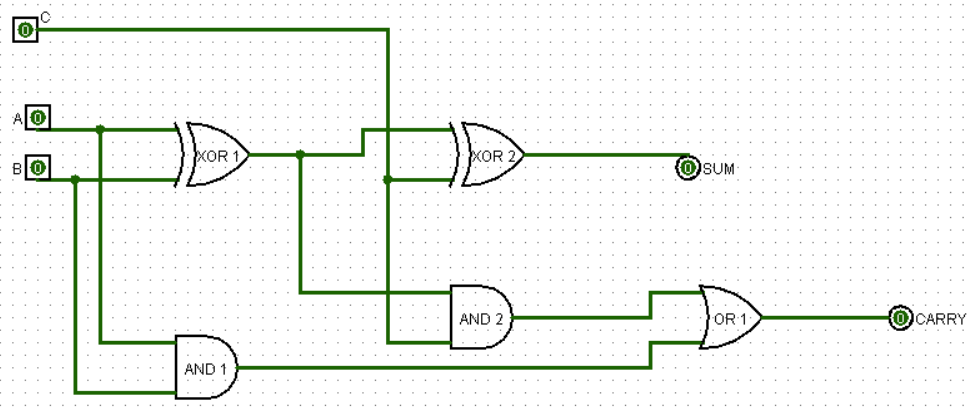
\includegraphics[scale=0.6]{circuito full-adder.png}
    \caption{Circuito Full-Adder}
\end{figure}

2. Organização do Pipeline:
Com a arquitetura definida, partimos para a organização do pipeline de cinco estágios. Cada estágio foi cuidadosamente projetado para executar uma etapa específica do processamento de instruções. O pipeline foi dividido em:

\begin{figure}[h]
    \centering
    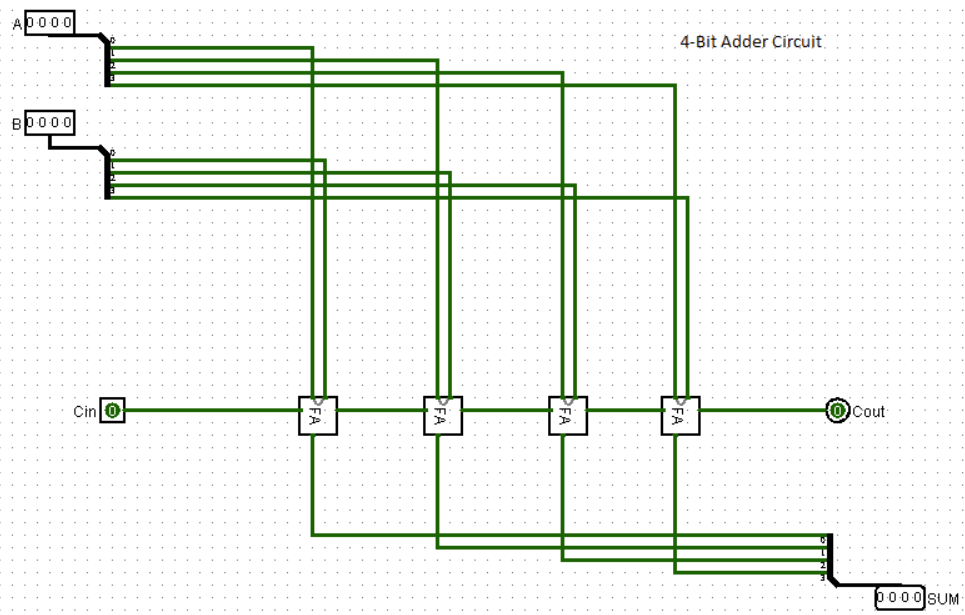
\includegraphics[scale=0.6]{circuito 4 bit adder.png}
    \caption{Circuito 4-Bit Adder}
\end{figure}

Estágio de Busca de Instrução (IF): Responsável por buscar a instrução na memória de instruções (IMEM) e encaminhá-la para o próximo estágio.
Estágio de Decodificação de Instrução (ID): Realiza a decodificação da instrução buscada, identificando o tipo da operação e os operandos envolvidos.
Estágio de Execução (EX): Efetua a execução da operação com base nos operandos decodificados, gerando os resultados necessários para a próxima etapa.
Estágio de Acesso à Memória (MEM): Responsável por acessar a memória de dados (DMEM) quando necessário, para operações de carga e armazenamento de dados.
Estágio de Escrita de Resultados (WB): Escreve os resultados finais no banco de registradores.
3. Implementação dos Blocos em VHDL:
Com a organização do pipeline definida, partimos para a implementação dos blocos funcionais em VHDL. Cada estágio do pipeline foi modelado como um bloco independente, permitindo modularidade e facilitando a manutenção do código. Foram implementados os blocos para a busca de instrução, decodificação, execução, acesso à memória e escrita de resultados.

4. Memórias de Instruções e Dados:
Para suportar a carga assíncrona de dados, as memórias de instruções (IMEM) e dados (DMEM) foram modificadas. A abordagem de leitura de palavras por ciclo foi adotada para otimizar a busca de instruções e o acesso à memória de dados. Além disso, foram incluídos mecanismos de controle para pausar a operação da CPU durante a carga assíncrona de dados e evitar conflitos de leitura e escrita.

\begin{figure}[h]
    \centering
    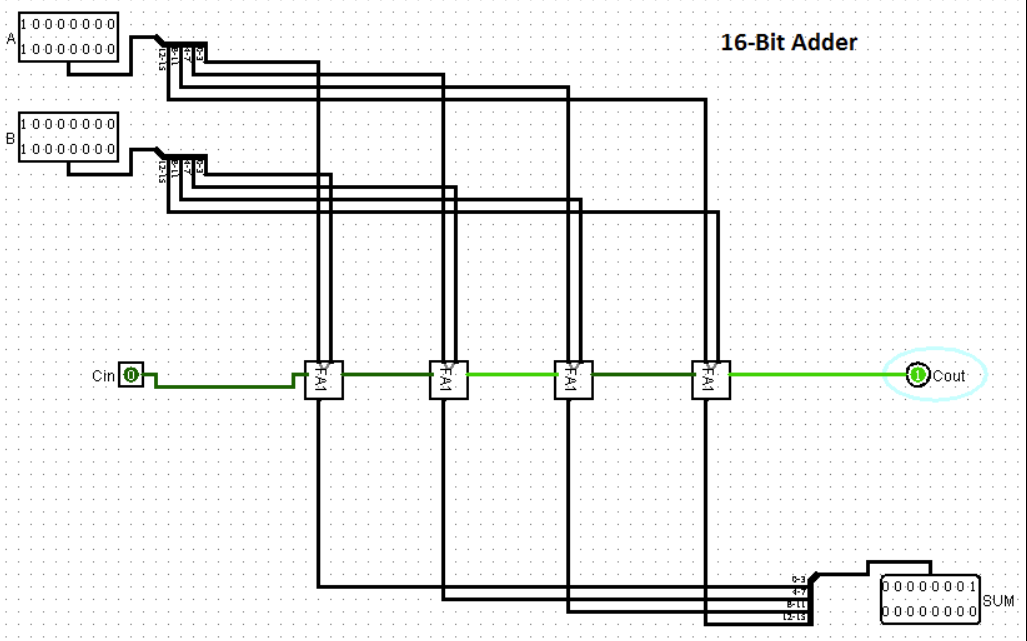
\includegraphics[scale=0.6]{Circuito 16 bit adder.png}
    \caption{Circuito 16-Bit Adder}
\end{figure}


5. Testes e Validação:
Após a implementação dos blocos em VHDL, foram realizados testes e validações em cada estágio do pipeline, garantindo que as instruções fossem decodificadas e executadas corretamente. Testvectors foram criados para simular diferentes cenários de execução, incluindo casos de teste com operações aritméticas, lógicas, saltos, ramificações e acesso à memória.

\newpage
\newpage

\begin{figure}[h]
    \centering
    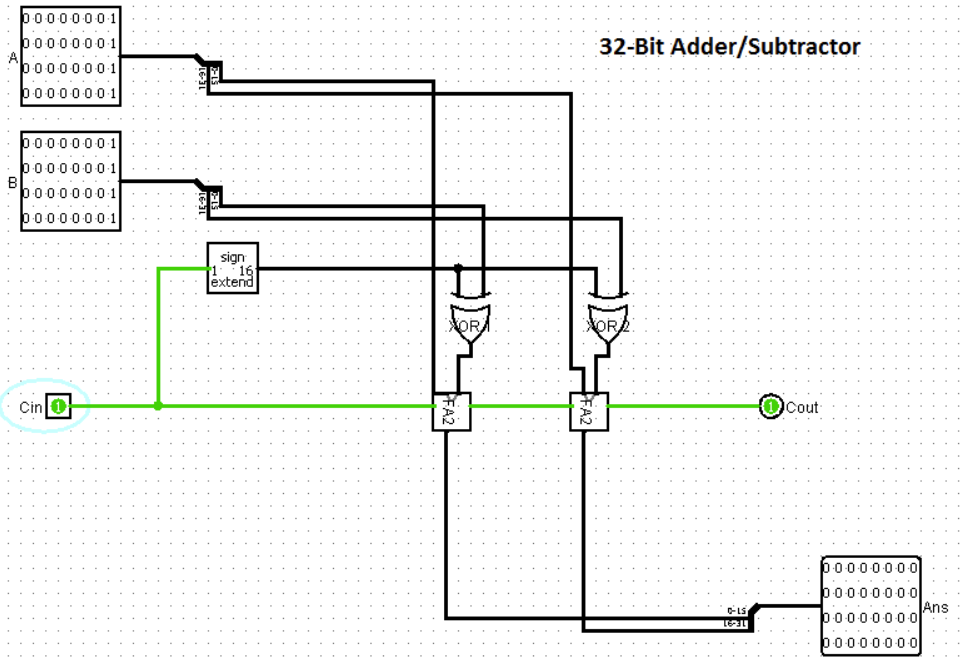
\includegraphics[scale=0.6]{circuito 32 bit adder.png}
    \caption{Circuito 32-Bit Adder/Subtractor}
\end{figure}

6. Integração e Verificação do Pipeline:
Em seguida, todos os blocos foram integrados para formar o pipeline completo. A interação entre os estágios foi verificada, garantindo que as instruções fossem processadas corretamente ao longo do pipeline. Foram realizados testes abrangentes para verificar o correto encaminhamento de dados entre os estágios e a correta execução das instruções suportadas.

7. Implementação da Unidade de Controle:
Uma parte essencial da CPU é a unidade de controle, responsável por coordenar todas as etapas do pipeline e garantir o funcionamento correto da CPU em resposta às instruções recebidas. A unidade de controle foi projetada e implementada em VHDL para gerenciar o fluxo de dados e controlar as operações de carga assíncrona, pausando e retomando a execução da CPU conforme necessário.

8. Verificação do Funcionamento Global:
Após a implementação da unidade de controle, a CPU foi novamente testada e validada em sua totalidade, garantindo que todas as instruções suportadas fossem corretamente executadas. Foram realizados testes mais extensivos para avaliar o desempenho da CPU sob diferentes cargas de trabalho e cenários de execução.

\subsection{Código VHDL Full-Adder}

\begin{lstlisting}
library IEEE;
use IEEE.STD_LOGIC_1164.ALL;



entity FullAdder is
    Port ( x : in  STD_LOGIC;
           y : in  STD_LOGIC;
           cin : in  STD_LOGIC;
           cout : out  STD_LOGIC;
           sum : out  STD_LOGIC);
end FullAdder;

architecture Behavioral of FullAdder is

begin
sum <= x xor cin xor y;
cout <= (x and y) or (y and cin) or (x and cin);

end Behavioral;
\end{lstlisting}

\subsection{Código VHDL Full-Adder}
\begin{lstlisting}
library IEEE;
use IEEE.STD_LOGIC_1164.ALL;


entity Adder_32_bits is
    Port ( A : in  STD_LOGIC_VECTOR (31 downto 0);
           B : in  STD_LOGIC_VECTOR (31 downto 0);
           Ci : in  STD_LOGIC;
           S : out  STD_LOGIC_VECTOR (31 downto 0);
           Co : out  STD_LOGIC);
end Adder_32_bits;

architecture Behavioral_artch of Adder_32_bits is

component FullAdder is
    Port ( x : in  STD_LOGIC;
           y : in  STD_LOGIC;
           cin : in  STD_LOGIC;
           cout : out  STD_LOGIC;
           sum : out  STD_LOGIC);
end FullAdder;

begin

signal C : std_logic_vector ( 31 downto 1);

FA0 : FullAdder port map ( A(0),B(0),Ci,C(1),S(0) );
FA1 : FullAdder port map ( A(1),B(1),C(1),C(2),S(1) );
FA2 : FullAdder port map ( A(2),B(2),C(2),C(3),S(2) );
FA3 : FullAdder port map ( A(3),B(3),C(3),C(4),S(3) );
FA4 : FullAdder port map ( A(4),B(4),C(4),C(5),S(4) );
FA5 : FullAdder port map ( A(5),B(5),C(5),C(6),S(5) );
FA6 : FullAdder port map ( A(6),B(6),C(6),C(7),S(6) );
FA7 : FullAdder port map ( A(7),B(7),C(7),C(8),S(7) );
FA8 : FullAdder port map ( A(8),B(8),C(8),C(9),S(8) );
FA9 : FullAdder port map ( A(9),B(9),C(9),C(10),S(9) );
FA10 : FullAdder port map ( A(10),B(10),C(10),C(11),S(10) );
FA11 : FullAdder port map ( A(11),B(11),C(11),C(12),S(11) );
FA12 : FullAdder port map ( A(12),B(12),C(12),C(13),S(12) );
FA13 : FullAdder port map ( A(13),B(13),C(13),C(14),S(13) );
FA14 : FullAdder port map ( A(14),B(14),C(14),C(15),S(14) );
FA15 : FullAdder port map ( A(15),B(15),C(15),C(16),S(15) );
FA16 : FullAdder port map ( A(16),B(16),C(16),C(17),S(16) );
FA17 : FullAdder port map ( A(17),B(17),C(17),C(18),S(17) );
FA18 : FullAdder port map ( A(18),B(18),C(18),C(19),S(18) );
FA19 : FullAdder port map ( A(19),B(19),C(19),C(20),S(19) );
FA20 : FullAdder port map ( A(20),B(20),C(20),C(21),S(20) );
FA21 : FullAdder port map ( A(21),B(21),C(21),C(22),S(21) );
FA22 : FullAdder port map ( A(22),B(22),C(22),C(23),S(22) );
FA23 : FullAdder port map ( A(23),B(23),C(23),C(24),S(23) );
FA24 : FullAdder port map ( A(24),B(24),C(24),C(25),S(24) );
FA25 : FullAdder port map ( A(25),B(25),C(25),C(26),S(25) );
FA26 : FullAdder port map ( A(26),B(26),C(26),C(27),S(26) );
FA27 : FullAdder port map ( A(27),B(27),C(27),C(28),S(27) );
FA28 : FullAdder port map ( A(28),B(28),C(28),C(29),S(28) );
FA29 : FullAdder port map ( A(29),B(29),C(29),C(30),S(29) );
FA30 : FullAdder port map ( A(30),B(30),C(30),C(31),S(30) );
FA31 : FullAdder port map ( A(31),B(31),C(31),Co,S(31) );


end Behavioral_artch;
\end{lstlisting}

\subsection{Código Programa Principal}

\begin{lstlisting}
LIBRARY ieee;
USE ieee.std_logic_1164.ALL;
 
-- Uncomment the following library declaration if using
-- arithmetic functions with Signed or Unsigned values
--USE ieee.numeric_std.ALL;
 
ENTITY adder_32_bit_adder IS
END adder_32_bit_adder;
 
ARCHITECTURE behavior OF adder_32_bit_adder IS 
 
    -- Component Declaration for the Unit Under Test (UUT)
 
    COMPONENT Adder_32_bits
    PORT(
         A : IN  std_logic_vector(31 downto 0);
         B : IN  std_logic_vector(31 downto 0);
         Ci : IN  std_logic;
         S : OUT  std_logic_vector(31 downto 0);
         Co : OUT  std_logic
        );
    END COMPONENT;
    

   --Inputs
   signal A : std_logic_vector(31 downto 0) := (others => '0');
   signal B : std_logic_vector(31 downto 0) := (others => '0');
   signal Ci : std_logic := '0';

 	--Outputs
   signal S : std_logic_vector(31 downto 0);
   signal Co : std_logic;
   -- No clocks detected in port list. Replace <clock> below with 
   -- appropriate port name 
 
   constant period : time := 10 ns;
 
BEGIN
 
	-- Instantiate the Unit Under Test (UUT)
   uut: Adder_32_bits PORT MAP (
          A => A,
          B => B,
          Ci => Ci,
          S => S,
          Co => Co
        );


 

   -- Stimulus process
   stim_proc: process
   begin		
    A <= "10101001101010101010001010101011";

B <= "10101001101010101010001010101010";

Ci <= '0';

      wait;
   end process;

END;
\end{lstlisting}

\section{Resultados}

\begin{figure}[h]
    \centering
    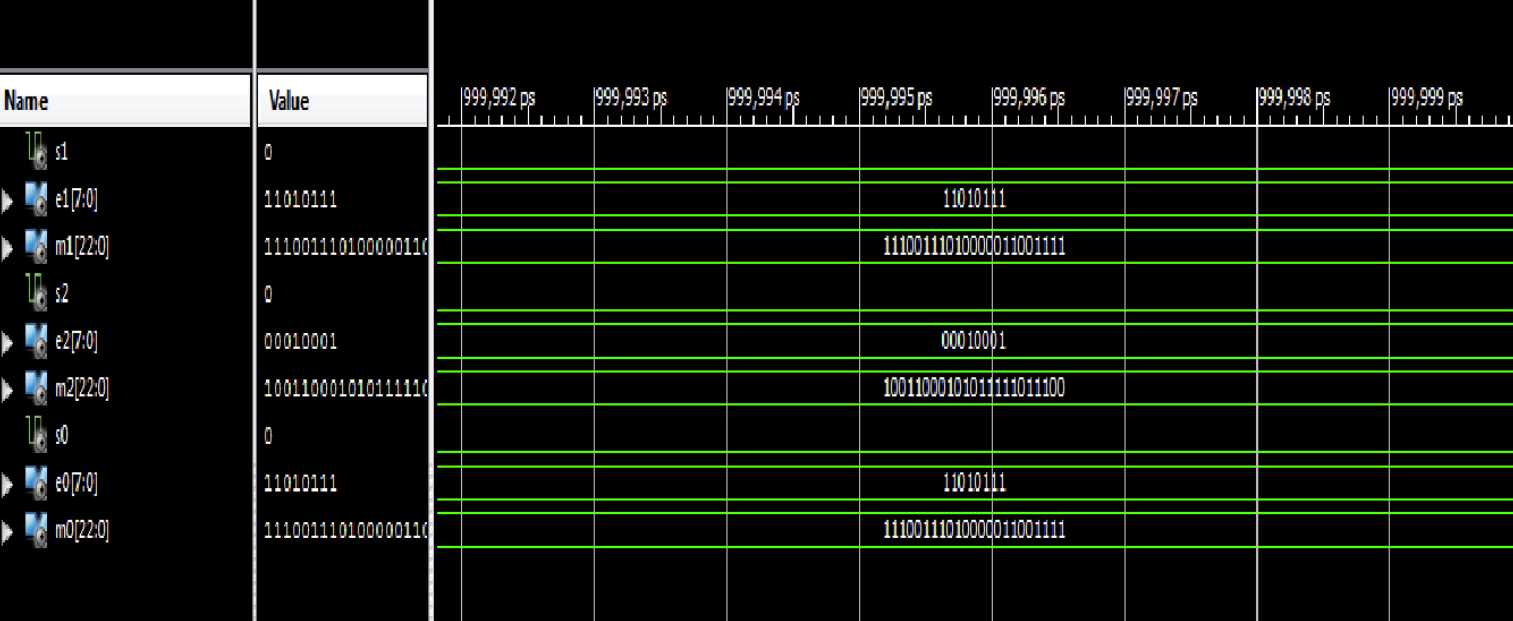
\includegraphics[scale=0.6]{simulação cpu 32 bits adição.png}
    \caption{Simulação cpu 32 bits adição}
\end{figure}

\begin{figure}[h]
    \centering
    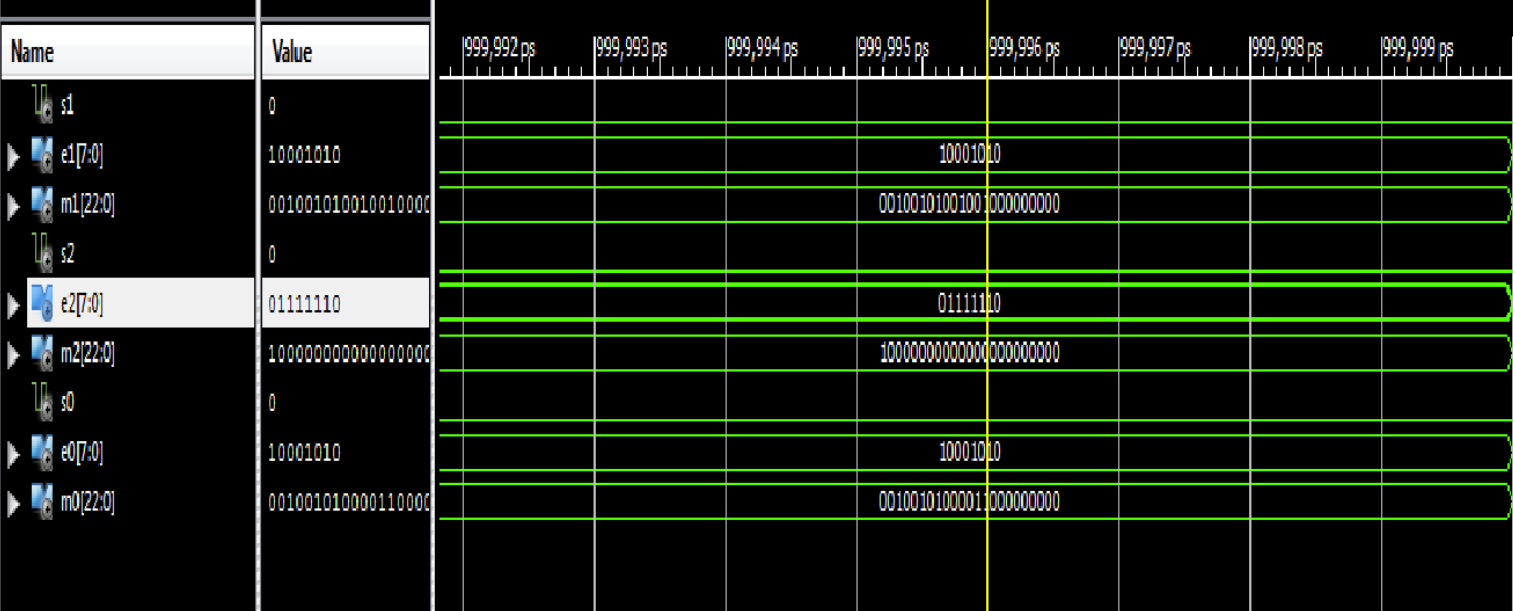
\includegraphics[scale=0.6]{simulação cpu 32 bits subtração.png}
    \caption{Simulação cpu 32 bits subtração}
\end{figure}

\newpage
\newpage

\subsection{Conclusão}
Uma análise de desempenho foi realizada para avaliar a eficiência do pipeline de cinco estágios em relação ao throughput e à latência de execução. Foram identificados gargalos e possíveis melhorias para otimizar ainda mais o desempenho da CPU.

Portanto, o desenvolvimento deste projeto resultou na implementação de uma CPU funcional baseada na arquitetura RISC-V de 32 bits, com um pipeline de 5 estágios. A CPU suporta um conjunto seleto de instruções do RV32I, permitindo operações inteiras e demonstrando um desempenho otimizado através da técnica de pipeline. A modificação das memórias para permitir a carga assíncrona de dados, juntamente com a implementação da unidade de controle, possibilitou o funcionamento contínuo da CPU durante esse processo.

O projeto proporcionou uma experiência enriquecedora no desenvolvimento de uma CPU RISC-V, explorando conceitos fundamentais de microarquitetura, pipeline e controle de CPU. Embora tenhamos obtido sucesso na implementação do pipeline de inteiros, reconhecemos que existem oportunidades para aprimorar ainda mais a CPU, expandindo o suporte a mais instruções e incorporando unidades funcionais adicionais.

\section{Referências}

\begin{enumerate}
\item \textit{Computer Organization and Design RISC-V Edition: The Hardware Software Interface}, 2nd edition, by David A. Patterson and John L. Hennessy. Morgan Kaufmann, 2021.

\item \textit{Computer Organization and Architecture: Designing for Performance}, 11th edition, by William Stallings. Pearson, 2022.

\item \textit{Digital Design Using VHDL: A Systems Approach} by John F. Wakerly. Pearson, 2016.

\end{enumerate}

\end{document}